% !TEX root = ../main.tex

\chapter{Proof construction}
In this chapter we will construct the proof of liabilities and proof of inclusion. We will go through different circuit designs to find the optimal proof of inclusion and proof of liabilities.
We will be working with a proof of inclusion derived from existing literature, and a novel proof of liabilities.

\section{Constants}
Before constructing the circuits, we need to define the constants that will be shared between the
different circuits.


\subsection{Circom} 

Circom is a domain-specific language designed for creating arithmetic circuits, specifically utilized in zk-SNARKs. These proofs verify calculations without revealing private data, like proving you have funds without showing your account.
Within Circom, circuit code is written to define the desired constraints. One notable distinction from other languages is the utilization of signals and templates.
Templates can be conceptualized as functions that operate as circuits. The primary template receives signals as inputs and produces other signals as outputs. Signals can be classified as either public or private.
Assigning a value to a signal contributes to the constraint system and the witness calculation process.
Input and outputs are signals, and you can have additional intermediate signals.
During circuit compilation, constraints are generated in r1cs format. Additionally, compiling a circuit produces a witness file containing the data essential for verifying the constraints and demonstrating the correct behavior of the circuit.

\subsection{MiMCSponge} 
MiMCSonge is a standard hashing algorithm often used in zero knowledge protocols. It was chosen because it is secure and well integraded with circom.
The hash function is $F_i(x) = (x + k + c_i)^3$, where $i$ is the number of round, $k$ a fixed constant, and $c_i$ a constant that is specific for a round.
In our implementation, we use $i = 220$ and $k = 1$, which are both standard values. We use 4 inputs, the two sums and two hashes of the children. 
The hash function is a sponge construction, which means that it can take any number of inputs and produce any number of outputs. It does the 220 rounds on the first input, then add the second input and start over again.


\subsection{Constraints} 

A zero knowledge circuit has generally two types of constraints: range check and arithmetic.
The simple arithmetic case is when we define a value in Circom $a = b + c$. Circom compiled the assignment to create an arithmetic constraint that verifies the equality.

A range check verifies that a value lies within specified bounds. This is needed because we are working in a finite field. This means that an overflow would cause the value to go back to 0.
We limit the range of the values to make sure we never have any overflow. This is critical because an overflow would change the balance sum, which is what we are trying to prove.

In Circom, the range check constraint is transform to be arithmetic as well. For example, to check $x<n$, we would use a library function $lessThan$.
The function decomposes the numbers in bits, and then does a series of bit equality to determine the result. The bit equalities are compiled by Circom in arithmetic constraints.

In Circom, we use a specific type of variable type called a signal. Usually when we assign a value to a signal, a constraint is created.
There is a way to assign value without creating a constraint, but it adds complexity and we never use it in this paper. 
Therefore it is safe to assume that every time we assign a value to a signal, we create a constraint. 
Every variables in this chapter will be of the type signal.
This means that the values will be constrained automatically as we define them. 


\subsection{SnarkJS} 

SnarkJS is a JavaScript library that provides tools for working with zk-SNARKs, including circuit compilation.
SnarkJS facilitates generating zk-SNARK proofs for specific instances of the circuit using the r1cs and witness file.
SnarkJS also provides utilities for verifying the proofs.

\subsection{Benchmark} 
We use Groth16 as a SNARK design choice because it is simple and fast. 
We will benchmark the circuits using the prover time and verifier time. The prover time does not include the time to generate the setup.
The setup needs to be generated for every circuit, but it only needs to be generated once. This is why we exlucde it from our benchmarks.
The prover time is the time to generate the proof, which includes generating the constraints, and folding them when we are using the folding schene. 
The verifier time is the time to verify the proof.

\subsection{Tree construction}
The size of the tree is dynamic with the number of users. For instance if we have $2^5 - 10$ users, we will use a tree of 5 levels. This means we will
have 10 empty nodes. We will use empty hash and 0 as the value for the empty nodes. Those values are valid inputs for the MiMCSponge hash construction,
and will give a valid hash has an output. An empty node has no impact on the state of the tree.

The size of the tree decides the number of constraints. We need a separate setup for every tree size, but they those setups are precomputed. 
For instance, a power of Tau of 8 (8 refers to the number of degree of the QAP polynomial) can handle up to 256 constraints, 9 for 512 constraints, and so on.


\section{Proof of liabilities}
\label{subsec:pl}
The proof of liabilities operates on a list of balances and a list of email hashes as private inputs.
The first purpose of the circuit is to validate that all values are non-negative and that all balances fall within a specified range.
These verifications are crucial to prevent overflow or underflow issues, given that the operations occur within a finite field. 
The circuit sums balances, checks ranges, and builds a Merkle tree by repeatedly combining values with a secure scrambling process called hashing, which is complex to ensure privacy.

Subsequently, the proof of liabilities constructs a Merkle tree and outputs the total balance sum and the root hash of the Merkle tree.
The pseudocode for the circuit is found \hyperref[subsec:plc]{here}.


\paragraph{Inputs}
\begin{itemize}
   \item List of balance (private): List of user balances, kept secret to protect individual amounts.
   \item List of email hash (private): User emails, hidden to protect identities and used in the Merkle tree.
   \end{itemize}

\paragraph{Outputs}
\begin{itemize}
   \item Balance Sum : Total of all balances, showing overall liabilities without revealing individual amounts.
   \item Root hash: Merkle tree's top value, used to check the integrity of the tree.
   \item No negative values: True if all balances are zero or positive, ensuring valid data.
   \item All small range: True if balances are within a safe range, preventing math errors.
   \end{itemize}

This proof of liabilities operates as intended because it returns the sum of the liabilities, which is exact because of the verifications.
It also returns the root hash, ensuring you cannot alter any values inside the merkle tree. The merkle tree is hidden so that we do not
give any information about users and their balances.
The root hash will be used to verify the inclusion of the balances.

In a complete proof of reserves, the balance sum would be a private output. We would have another circuit proving that the sum of liabilities is smaller
than the sum of assets, without revealing the balance.

The circuit follow the zero knowledge \hyperref[subsec:zkp]{properties} we highlighted previously. 
\paragraph{Properties}
\begin{itemize}
   \item Completeness: If the input balances are non-negative and within the range, a Merkle sum tree will be produced alongside the proof. This is enforced by the arithmetic constraints and range checks.
   \item Soundness: If any input balance is negative or outside the range, a valid proof cannot be produced. Moreover, the Merkle sum tree cannot produce an inacurate root hash and sum if the inputs are valid due to constraints ensuring sum accuracy and Merkle path integrity.
   \item Zero-Knowledge: The verifier learns only the public outputs, from which he does not gain any information about the individual inputs. The hash provides not useful information.
   \end{itemize}


\section{Proof of inclusion}
\label{subsec:pi}
The proof of inclusion aims to prove that the balance of a user is included in the Merkle tree created in the proof of liabilities. 
It checks if a path through the tree leads to the correct top value, proving the balance is included without revealing other data.
To prove that a balance is included, it is sufficient to show that you know the Merkle path of a user balance,
which we define using the list of neighbors sum, hash and binary.
The neighbors binary variable indicates whether the neighbor is on the left or the right. The circuit combines the user's data with neighbors using hashing, a complex step ensuring correctness.
The root hash, root sum, user balance and user email hash are public because it needs to be shown which user is in which tree.

For the next figure, the blue nodes represent the value of the merkle path.
We would have $neighborsSum=[29,61]$, $neigborsHash=[Hash(User1),Hash(L2,R2)]$ and $neighborsBinary=[0,1]$.
   \begin{figure}[H]
   \centering
   \includegraphics[width=130mm]{MerklePath.png}
   \caption{Merkle Path}
   \label{overflow}
   \end{figure}

\paragraph{Inputs}
\begin{itemize}
   \item List of neighbors sum (private): Sums of nearby tree nodes, kept secret to hide the tree's structure.
   \item List of neighbors hash (private): Hash value of nearby nodes, hidden for privacy.
   \item List of neighbors binary (private): Value showing if a neighbor is left (0) or right (1).
   \item Root hash (public): Merkle tree's top value, shared to identify the tree.
   \item Root sum (public): Total balance sum, shared for verification.
   \item User balance (public): User's balance, shared to prove it's included.
   \item User email hash (public): User email hash, shared to identify the user.
   \end{itemize}

\paragraph{Outputs}
\begin{itemize}
   \item balanceIncluded: True if the balance is in the Merkle tree, confirming it's part of the data.
   \end{itemize}



The constraints in the circuit ensure the path from the leafs to the root is correct. 
In the \hyperref[subsec:pic]{circuit}, we verify that the combination of the user balance, sum, and Merkle path gives the right root hash and root sum. 
The circuit iterates over the path, combining values to recompute the root without revealing private data. 
There is no additional verifications since they are already done for this root hash, in the proof of liabilities. 
Constraints enforce the hash and sum calculations and path directions. 
Each new value in Circom is defined in a way that adds a constraint. For instance the Root sum is constrained to be equal to its two childs, the childs are constrained to be equal to their two childs, and so on.

Once again, the circuit follow the zero knowledge \hyperref[subsec:zkp]{properties}. 
\paragraph{Properties}
\begin{itemize}
   \item Completeness: If a user's balance and email hash are included in the Merkle tree, an honest prover can provide a valid Merkle path. This is verified by recomputing with constraints the public root hash and sum.
   \item Soundness: If the user's balance or email hash is not in the Merkle tree, or if the Merkle path is incorrect, no dishonest prover can produce a valid proof. This is because the hash function is collision resistant.
   \item Zero-Knowledge: The verifier only learns wheter the user's balance is included in the Merkle tree, and nothing about the private inputs. All of the tree internal structure is preserved with the SNARK privacy properties.
   \end{itemize}

\section{Daily proof of liabilities}
We aim to enhance our current \hyperref[subsec:pl]{circuit} by minimizing the work needed in subsequent rounds.
The first thing to explore is recursion proofs, as they were specifically created to reduce the total computational effort across rounds.

\subsection{Aggregation proofs}
The main advantage of the aggregation proof is in streamlining the verification process. For instance, in the second round, we can prove the integrity of the current round and all previous rounds.
However, this benefit comes with trade-offs. The first drawback is the increase in proof size, as it necessitates to prove the current circuit and verify the previous ones.
When considering the frequency of verification, having a fixed number of nodes verify the proof daily, it would be illogical to make the nodes verify the previous rounds every single day.
On the other hand, if the verification is not consistent, or there is a need for new nodes to be able to come in and verify every proof quickly, then aggregation becomes more appealing.

In our case, the priority is to produce daily succinct proofs. We need to ensure the integrity of every round, while keeping the proof size to a minimum.
Therefore, having our nodes verify the circuit at every round without the computational overhead of the aggregated proof is sufficient.

\subsection{Other recursion proofs}
The aggregation proof stands out as the only recursion proof potentially useful in certain scenarios.
If we examine the other types of recursion proofs, namely Recursion scheme, accumulation, and Folding scheme, they all have one thing in common.
They are all designed to verify multiple rounds concurrently.
This approach is not aligned with our objectives. We are interested in working on rounds independently and reducing the individual workload.

\subsection{Change circuit}
If we cannot use any recursion schemes, we need an alternative approach to reduce the complexity of subsequent rounds.
Our solution is to reutilize the same Merkle tree as the previous rounds, modify and adapt it to include the changes.
The key challenge is that the Merkle tree was built inside the circuit, and is therefore not accessible.

What we will be doing, in our modified circuit, is adjust the Merkle tree inside the circuit.
For every change, we send the corresponding Merkle path which will be verified by the circuit.
The circuit will then compute a new Root Hash for each change and output the final Merkle Hash. 
Internally, the circuit iterates over each change, verifies the old path, updates the leaf with new values, and recomputes the hash and sum up the tree.

The standard verification will be applied to the new values (e.g., non-negative values, limited range).
The constraints ensure correct hash and sum updates, valid path directions and valid ranges.

\paragraph{Inputs}
\begin{itemize}
   \item List of old email hash (private) - 1 per change: Hashed email addresses from the previous Merkle tree, kept secret to protect user identities.
   \item List of old values (private) - 1 per change: Previous balances, hidden to maintain user privacy.
   \item List of new email hash (private) - 1 per change: Updated hashed email addresses, kept secret to ensure user confidentiality.
   \item List of new values (private) - 1 per change: Updated balances, hidden to safeguard individual amounts.
   \item List of temporary root hash (private) - 1 per change: Intermediate Merkle tree top values, kept secret to conceal tree updates.
   \item List of temporary root sum (private) - 1 per change: Intermediate total balance sums, hidden to preserve privacy.
   \item Old root hash (public): Previous Merkle tree's top value, shared to verify the starting tree.
   \item Old root sum (public): Previous total balance sum, shared to confirm the initial sum.
   \item List of neighbors sum (private) - 1 list per change: Sums of nearby nodes in Merkle paths, kept secret to hide tree structure.
   \item List of neighbors hash (private) - 1 list per change: Hashed nearby nodes in Merkle paths, hidden to ensure privacy.
   \item List of neighbors binary (private) - 1 list per change: Left/right indicators (0 or 1) for Merkle paths, kept secret to protect path details.
\end{itemize}

\paragraph{Outputs}
\begin{itemize}
   \item Valid hash: True if the new Merkle hash is correct, confirming tree integrity.
   \item Valid sum: True if the new sum is correct, ensuring accurate totals.
   \item No negative values: True if new balances are zero or positive, ensuring valid data.
   \item All small range: True if new balances are within safe limits, to avoid overflow.
   \item New root hash : Final Merkle tree top value, used for future verifications.
   \item New root sum: Final total balance sum, reflecting updated liabilities.
   \end{itemize}

Here is an example of a change. In this case the change is a change in balance. First we prove that the 10 BTC of user 1 are
included in the merkle tree. Then we prove that the 11 BTC of user 1 are included in the new merkle tree. After the last change we are left
with the new root balance and the new root hash. Note that for every change we only need 1 merkle path.

\begin{figure}
   \hfill
   \subfloat[Pre change]{\includegraphics[width=70mm]{MerklePath.png}}
   \hfill
   \subfloat[Post change]{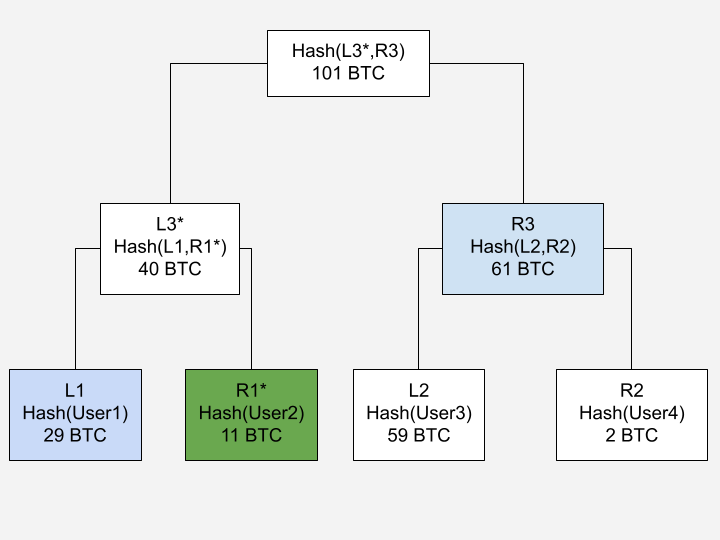
\includegraphics[width=70mm]{MerklePathTemp.png}}
   \hfill
   \caption{Merkle tree change}
   \end{figure}

For every change in the Merkle tree, we have the Merkle path with the old values, the new values, the temporary root hash, and the temporary root sum.
The \hyperref[subsec:plcc]{circuit} is iterating over the changes and gives a final root hash and final root sum. 
The circuit verifies each old path, updates the leaf with new values, and recomputes the hash and sum up the tree. 
The constraints enforce hash and sum calculations, valid path directions, and range checks.

The change circuit also follow the zero knowledge \hyperref[subsec:zkp]{properties}. 
\paragraph{Properties}
\begin{itemize}
   \item Completeness: If the changes are valid, with correct old and new Merkle paths, an honest prover can generate a proof that convinces an honest verifier of the statement. This is enforced by constraints on the paths and updates.
   \item Soundness: If any change is invalid, or if the old state is manipulated, no dishonest prover can produce a valid proof because of the constraints.
   \item Zero-Knowledge: The verifier learns only the public outputs and nothing about the private inputs.
   \end{itemize}

\subsubsection{Minimizing the number of changes}
To minimize the number of constraints, we want to minimize the number of changes.
We define a change as a hash change at the leaf level. Any new user, balance change, or removal of old user is considered as a change.
The naive change calculation would be $changes = balanceChanges + newUsers + deprecateUser$.
However, a new user can take the node of a deprecated user. So we would have the equation $changes = balanceChanges + max(newUsers, deprecateUser)$. 
Constraints enforce this calculation, reducing the circuit's complexity by limiting updates.

\subsubsection{Constraint analysis}
Theoretically, the new circuit makes sense. It should be quite faster than the original one, so let's analyze it.
We want to compare the number of constraints for the original circuit with the number of constraints with the change circuit.
The first assumption we are going to do, is to assume the number of changes in a day. A completely arbitrary value would be $1\%$.
\begin{figure}[H]
   \centering
   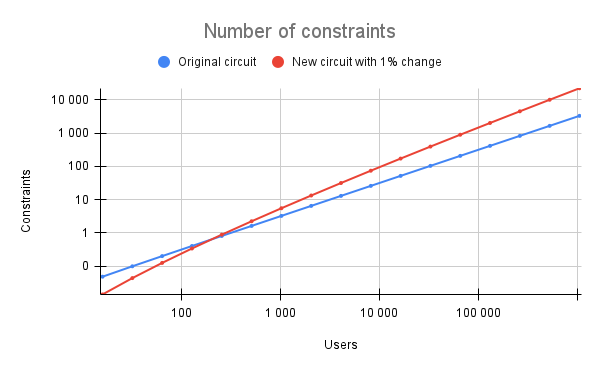
\includegraphics[width=130mm]{Number of constraints.png}
   \caption{Number of constraints original circuit vs new circuit with 1\% change}
   \label{overflow}
   \end{figure}
Once you reach more than 128 users with $1\%$ change, it is not worth it to use the new circuit.
This is not really practical because any marketplace will have more than 128 users.
However, we can see that the number of constraints of the new circuit grows linearly with the number of changes.
This means that two circuits of $0.5\%$ change would have a similar number of constraints as one circuit with $1\%$ change.
We can take this a step further and, instead of looking at daily proof, look at hourly proof.
Going with the assumption that $1\%$ change daily, we will assume that $0.05\%$ of the balances changes hourly.
Let's look at the number of constraints if $0.05\%$ of users change every hour.
\begin{figure}[H]
   \centering
   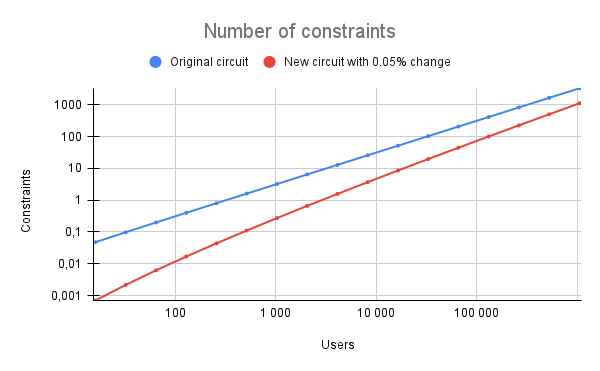
\includegraphics[width=130mm]{Number of constraints .05.png}
   \caption{Number of constraints (millions) original circuit vs new circuit with 0.05\% change}
   \label{overflow}
   \end{figure}
Even with more than 1 million users, there is still 3 times fewer constraints with our new circuit.
So if we want to do an hourly proof, it is less expensive with the new circuit than the old circuit.
We can take this a step further and do a proof at every new block. We could have a Merkle tree up to date for the liabilities side at every single block.

While the hourly proof and block proof is better with the new circuit, maybe a daily proof is sufficient for most use cases.
It is still less work to do the daily proof with the original circuit than to do 24 hourly proofs with the new circuit. 

\section{Daily proof of inclusion}
Because a marketplace can have millions of users, it is impractical to build a proof of inclusion for every single user on a daily basis.
It is the user's responsibility to request a proof that their balance is included in the published Merkle tree.

In an ideal world, a Merkle tree would be published at least daily. However, it is once again impractical to require every user to verify their inclusion every day.
Nevertheless, each user verifying their inclusion in the tree increases the chance that the proof of liabilities is valid and includes every single balance.
This is why it is primordial to find a way to make it easier to verify the inclusion. This is where Nova folding schemes come in.

The novel way to do proof of inclusion is to generate a proof of inclusion that is valid from the day of creation of the account to the requested day by the user.
Normally you would need to create 500 different proofs for 500 days. However, we saw in the previous section that the Nova folding scheme enables combining 500 proofs into just one.
The folding scheme circuit compresses multiple proofs by combining their constraints.
Verifying this one proof is the equivalent of verifying the 500, or any other number of days required.
This drastically simplifies the verification process.

Previously, when requesting a proof of inclusion, the user would only receive proof that their balance is included in the latest published Merkle tree. Now, the proof verifies that the balance has been included in every previously published Merkle tree. 
This ensures that any malicious entity would be unable to alter ownership of balances across multiple days. It might seem like a small detail, but it is the detail that makes all the difference, and here is why.

In this chart, we can observe the failure probability, which represents the likelihood that a dishonest prover gets away with misbehaving.
If we take for example the orange line, where an exchange has 1 million users, we notice that the failure probability approaches 0 when over $4\%$ of users perform their verifications.
However, without utilizing folding, this principle doesn't extend to every round. It implies that for each round, we require a minimum of $4\%$ of users to have a proof with significant confidence.

\begin{figure}[H]
   \centering
   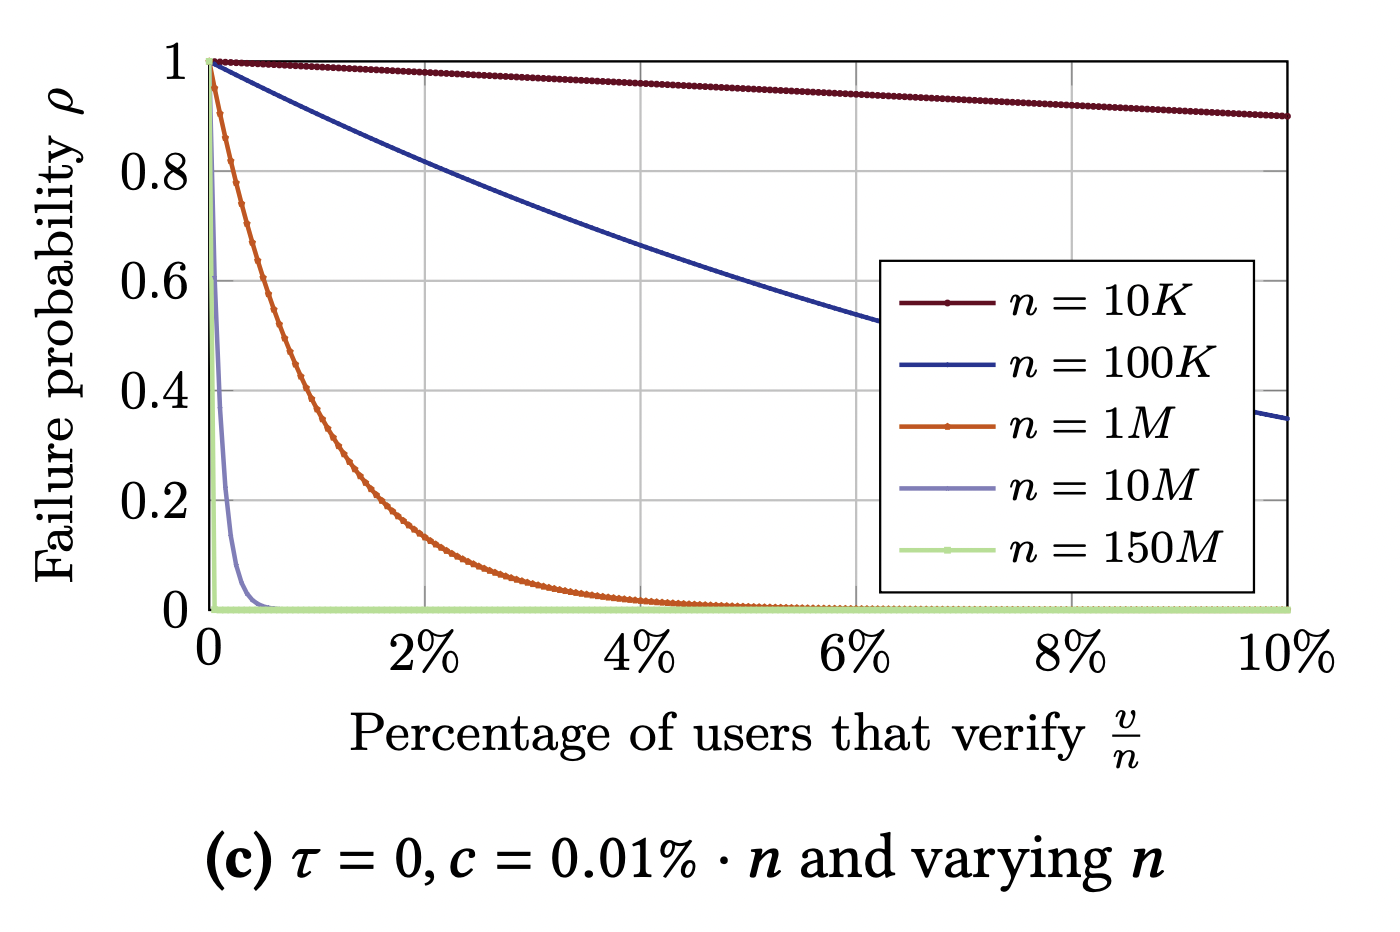
\includegraphics[width=130mm]{FailureProbability.png}
   \caption{Failure Probability \cite{GP21}}
   \label{overflow}
   \end{figure}

Now, let's evaluate the failure probability if we are using folding.
In the initial round, with no changes, the failure probability for 20k users remains at $13\%$.

\begin{figure}[H]
   \centering
   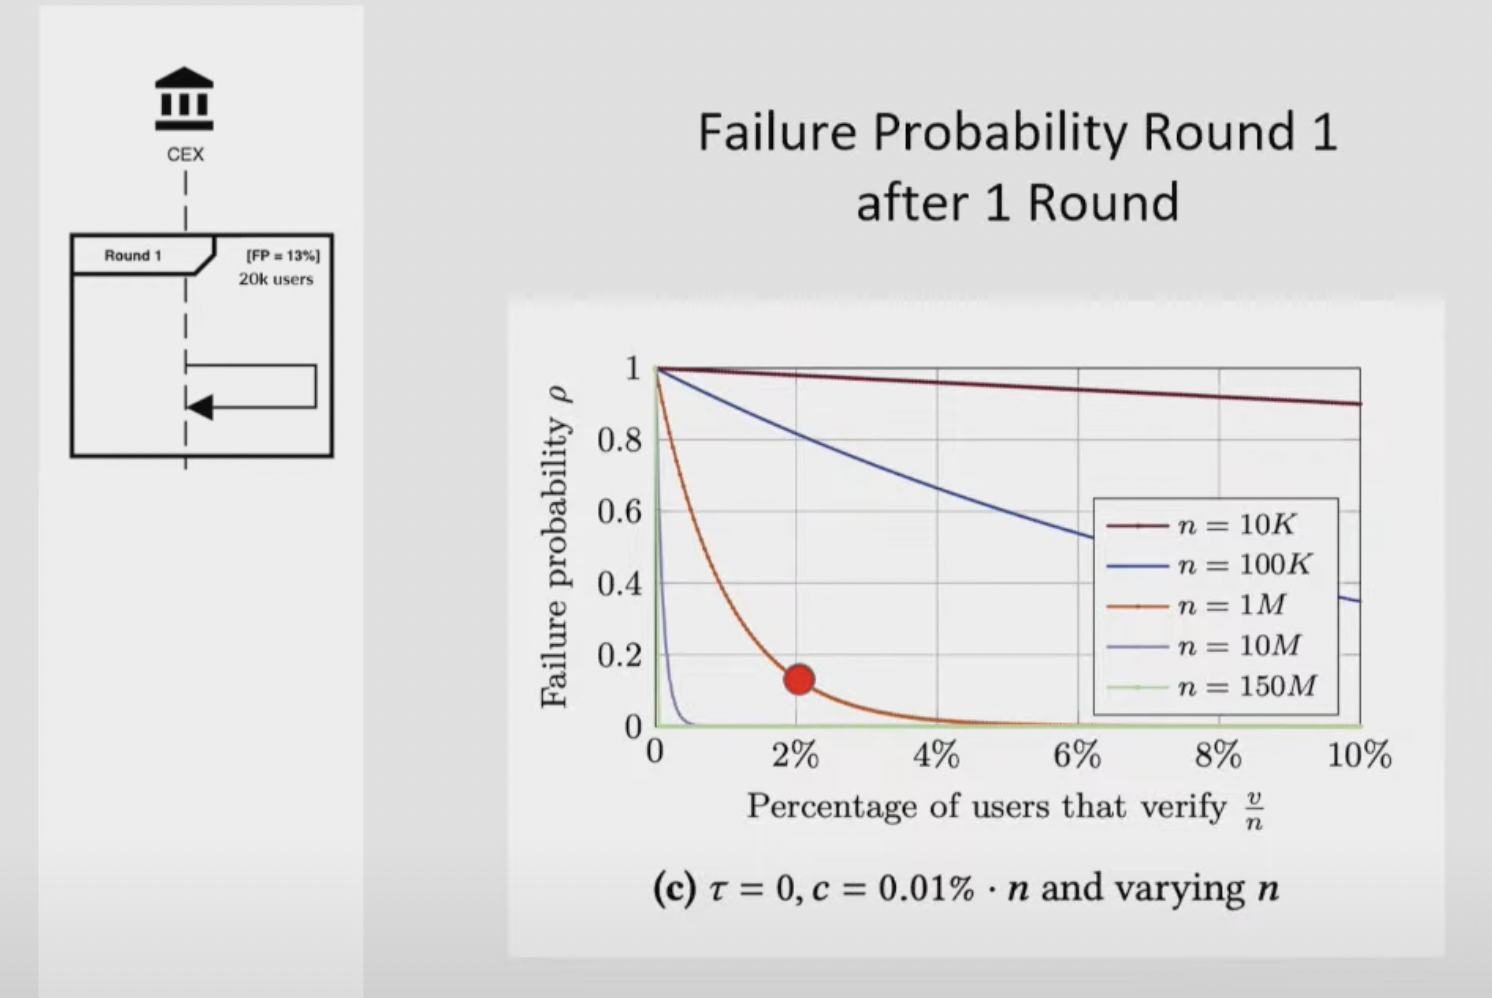
\includegraphics[width=130mm]{FailureProbabilityRound1.png}
   \caption{Failure Probability Round 1 \cite{NS23}}
   \label{overflow}
   \end{figure}

However, if we have 20k distinct users in round 2, the failure probability of round 1 decreases to $1.6\%$.

\begin{figure}[H]
   \centering
   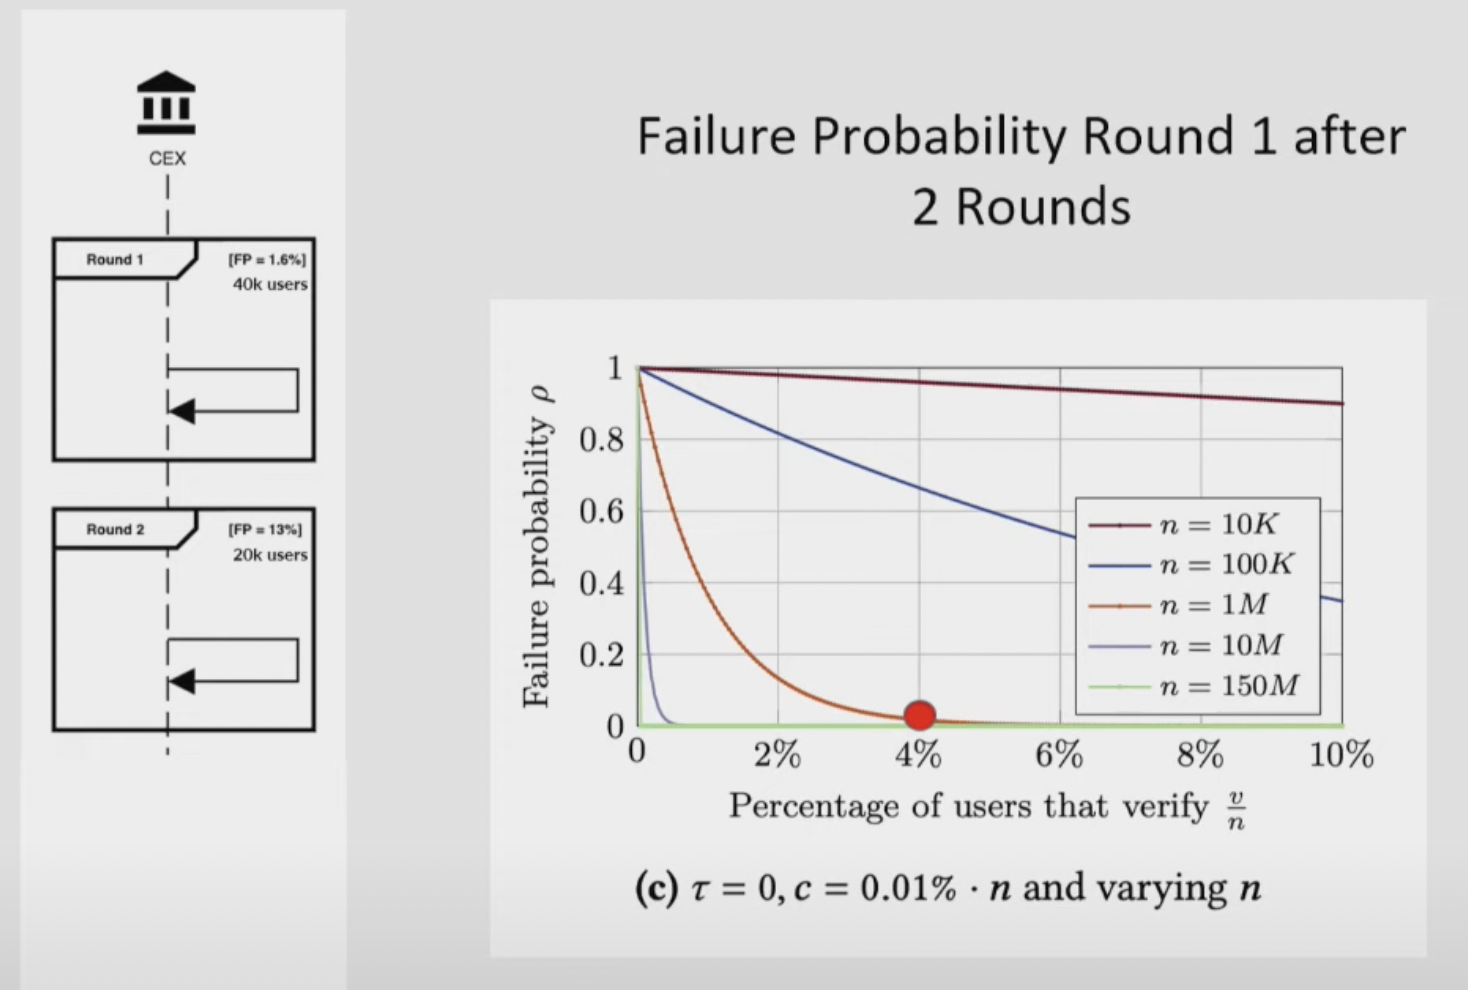
\includegraphics[width=130mm]{FailureProbabilityRound2.png}
   \caption{Failure Probability Round 1 After 2 Rounds \cite{NS23}}
   \label{overflow}
   \end{figure}

If we have 20k different users in round 3, the failure probability of round 1 further decreases to $0.2\%$.

\begin{figure}[H]
   \centering
   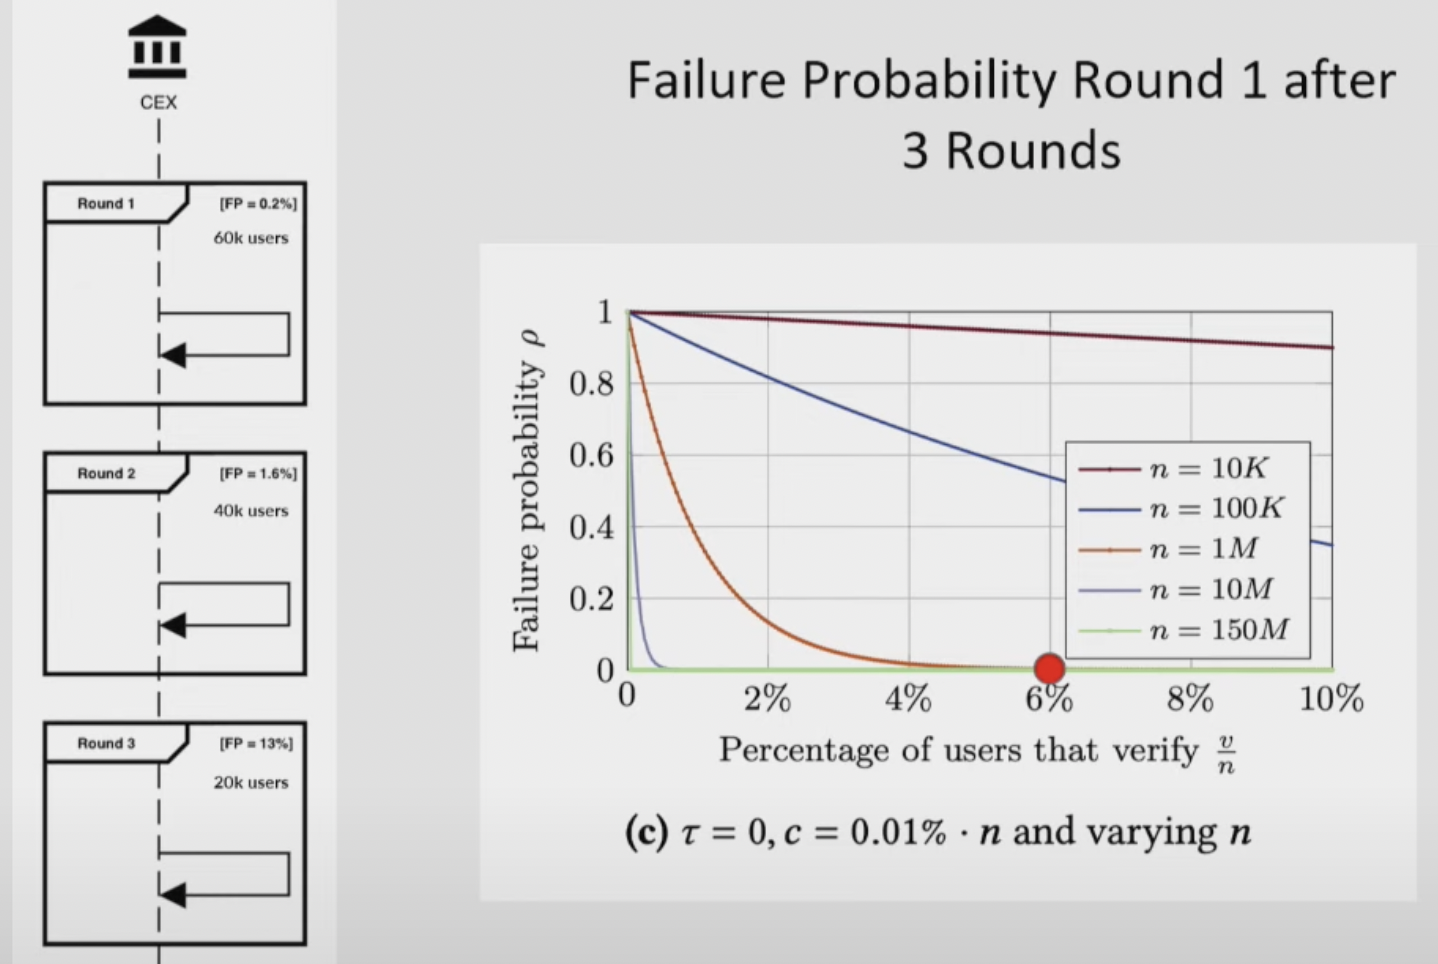
\includegraphics[width=130mm]{FailureProbabilityRound3.png}
   \caption{Failure Probability Round 1 after 3 Rounds \cite{NS23}}
   \label{overflow}
   \end{figure}
The key takeaway here is that without folding, you require $4\%$ of users to verify every round. However, with folding you only need
$4\%$ of users to participate in at least 1 round. This significantly reduces the burden on the user to verify, while increasing the confidence in the proof.

\subsection{Circuit Design}
The private inputs vary for each instance, whereas the public inputs are carried over from round to round.
In order to implement folding, we need to slightly adjust our \hyperref[subsec:pi]{circuit}. Everything except the way we handle inputs and outputs stays the same.
The private inputs vary for every instance, while the public inputs are carried over from round to round. 
The circuit verifies the Merkle path for a user's balance, recomputing the root hash and sum via hashing.

\paragraph{Inputs}
\begin{itemize}
   \item List of neighbors sum (private): Sums of nearby Merkle tree nodes, kept secret to hide the tree structure.
   \item List of neighbors hash (private): Hashed values of nearby nodes, hidden to protect tree privacy.
   \item List of neighbors binary (private): Left/right indicators (0 or 1) for the Merkle path, kept secret to conceal path details.
   \item Root hash (private): Merkle tree's top value, hidden to maintain proof privacy.
   \item Root sum (private): Total balance sum, kept secret to protect aggregate data.
   \item User balance (private): User's balance, hidden to preserve individual privacy.
   \item User email hash (private): Hashed user email, kept secret to protect identity.
   \item Steps in (public): Public values from the previous circuit's output, shared to link folded rounds.
   \end{itemize}

\paragraph{Outputs}
\begin{itemize}
   \item Steps out (public): Public values passed to the next circuit, enabling folding across rounds.
   \end{itemize}

\paragraph{Steps}
\begin{itemize}
   \item Balance included: Confirms the user's balance is in the Merkle tree.
   \item Root sum: Total balance sum for the tree.
   \item Root hash: Merkle tree's top value.
   \item User balance: User's balance value.
   \item User email hash: Hashed user email.
   \end{itemize}

All the data that is passed around between the circuits is public and is called step in and step out, and the regular inputs are private.
The step in of a circuit is the step out of the previous one.

\begin{figure}[H]
   \centering
   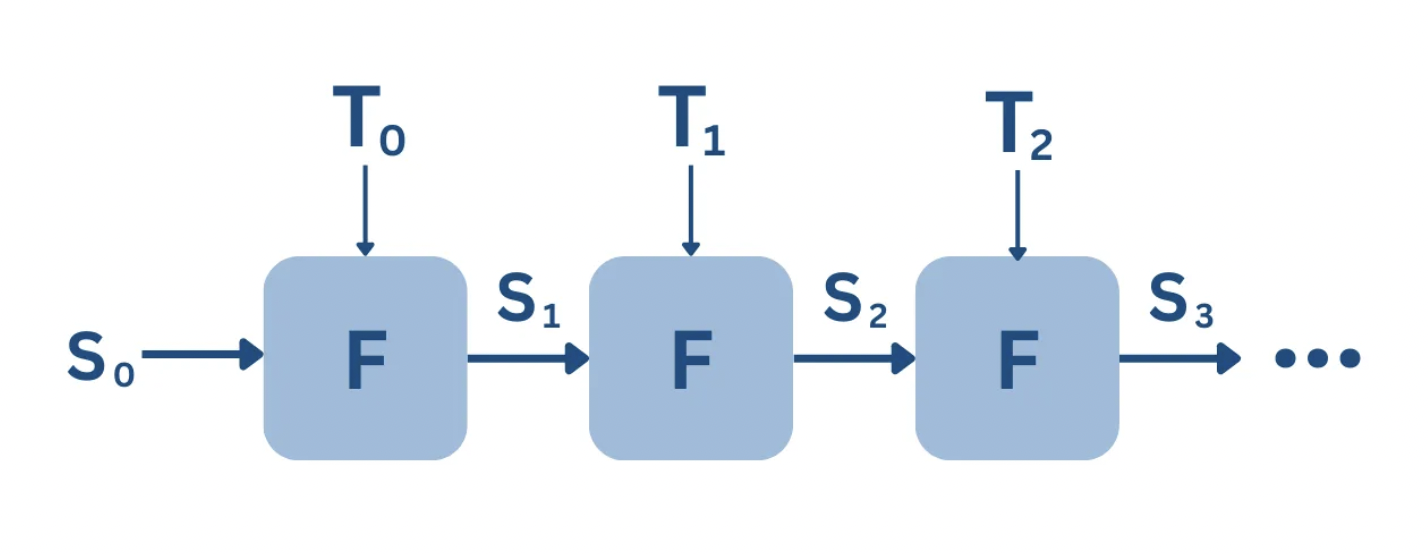
\includegraphics[width=130mm]{FoldingCircuit.png}
   \caption{Folding Circuit}
   \label{overflow}
   \end{figure}

S0 is the step in of the first change, S1 is the step out of first change and step in of second change. $F$ is the folded circuit
and $T$ is the number of times it is folded.

These steps encompass all the public values we initially had in the circuit.
None of the variables of the steps are used in the circuit itself. They are used as a means to make a value public.

The initial circuit takes meaningless values as inputs, while the following circuits take the public values of the previous circuit.
At the end you only have to verify a single proof. You also need to compare the circuit output with the proof of liabilities outputs for every round.

\section{Folded daily proof of liabilities}
With the original circuit, we saw how it was not useful to use folding or any other recursion scheme.
However, with the new circuit we saw that we were able to separate a big proof into multiple smaller ones.
This aligns perfectly with the recursion ideas.
We can separate our new circuit of $n$ changes into $m$ circuits, where $m <= n$, and fold the circuits together. 
The folding process combines constraints from each circuit.

\begin{figure}[H]
   \centering
   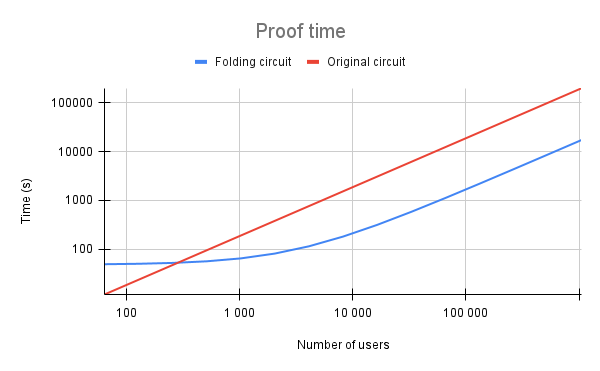
\includegraphics[width=130mm]{Proof time.png}
   \caption{Proof time original circuit vs folded circuit with 1\% change, 1 change by fold}
   \label{overflow}
   \end{figure}

As we can see, after 10 000 users, both circuits seem to be growing linearly, with the folded circuit doing much better. For instance,
at 1M users, we have the old circuit taking 196,608 seconds, and the new circuits taking 17 188 seconds. This is more than 10 times better.
We should take the number of seconds with a grain of salt, since these measurements were done on my Mac, and there are much more performant computers out there.
The data we should focus on is that it took 10x less time for the folded circuit, and it was not even optimized. We were doing 1 change by circuit, so at 1M users we folded 10k circuits.

Now that we know that our circuit is better, we can optimize it.

\begin{figure}[H]
   \centering
   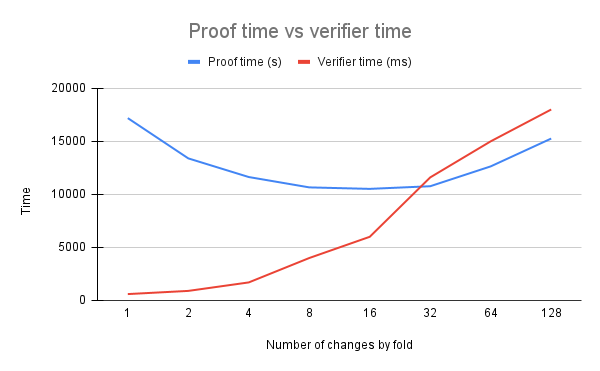
\includegraphics[width=130mm]{Proof time vs verifier time.png}
   \caption{Optimization of the proof time and verifier time of the folded circuit with 1\% change and 1M users}
   \label{overflow}
   \end{figure}

As we can see, the optimal time for the prover is between 8 and 32 changes by fold, while the verifier time seems to be growing at a monotonic pace.
Depending on the use case, you can decide the number of changes you should have for every fold.

\subsection{Circuit design}
The folded change circuit is exactly the same as the regular change circuit, but the inputs work differently because some data is passed around the circuits.
There are 2 types of step variables: the variables needed in the following circuit, and the variables that are just there to be public.
Starting from the inputs of the regular change circuit, the old hash and old sum root are moved to the step in, while all the outputs are moved to step out. 
The circuit processes each change by verifying old paths, updating leaves, and recomputing hashes and sums.

\paragraph{Inputs}
\begin{itemize}
   \item List of old email hash (private) - 1 per change: Hashed user email from the previous tree, kept secret to protect identities.
   \item List of old values (private) - 1 per change: Previous balances, hidden to preserve privacy.
   \item List of new email hash (private) - 1 per change: Updated hashed email, kept secret for user confidentiality.
   \item List of new values (private) - 1 per change: Updated balances, hidden to protect amounts.
   \item List of temporary root hash (private) - 1 per change: Intermediate tree top values, kept secret to hide updates.
   \item List of temporary root sum (private) - 1 per change: Intermediate balance sums, hidden for privacy.
   \item List of neighbors sum (private) - 1 list per change: Sums of nearby nodes in Merkle paths, kept secret to conceal tree structure.
   \item List of neighbors hash (private) - 1 list per change: Hashed nearby nodes in Merkle paths, hidden for privacy.
   \item List of neighbors binary (private) - 1 list per change: Left/right indicators (0 or 1) for Merkle paths, kept secret to protect path details.
   \item Step in (public): Public values from the previous circuit, shared to link folded circuits.
   \end{itemize}

\paragraph{Outputs}
\begin{itemize}
   \item Steps out: Public values passed to the next circuit, enabling folding.
   \end{itemize}

\paragraph{Steps}
\begin{itemize}
   \item Valid hash and valid sum: Confirms the new hash and sum are correct.
   \item No negative value and all small range: Ensures balances are non-negative and within safe limits.
   \item Root hash: Final Merkle tree top value.
   \item Root sum: Final total balance sum.
   \end{itemize}




%Mina proof of recursion
%summa
%https://summa.gitbook.io/summa/v/1/circuits/merkle-sum-tree-inclusion
%https://www.youtube.com/watch?v=sRAA1RYYHEs
%https://hackmd.io/@summa/HkGMF4Ovn#The-problem
